\documentclass[11pt]{amsart}

%Packages.

\usepackage[parfill]{parskip}
\usepackage{verbatim}
\usepackage{amsmath}
\usepackage{amssymb}
\usepackage{amsfonts}
\usepackage{amsthm}
\usepackage{mathrsfs}
\usepackage{tikz}
\usetikzlibrary{matrix,arrows}
\usepackage[all]{xy}
\usepackage{mathrsfs}
\usepackage{a4wide}
\usepackage{enumerate}
\usepackage{hyperref}
%\usepackage{showkeys}

%Theorem styles.

\theoremstyle{plain}
\newtheorem{conj}{Conjecture}
\newtheorem*{thm}{Theorem}
\newtheorem{theorem}{Theorem}%[section]
\newtheorem{lemma}[theorem]{Lemma}%[section]
\newtheorem{proposition}[theorem]{Proposition}%[section]
\newtheorem{corollary}[theorem]{Corollary}%[section]
\newtheorem{claim}[theorem]{Claim}%[section]
\newtheorem{question}[theorem]{Question}
\newtheorem{conjecture}[theorem]{Conjecture}


\theoremstyle{definition}%[section]
\newtheorem{definition}[theorem]{Definition}%[section]
\newtheorem{example}[theorem]{Example}%[section]
\newtheorem{project}{Project}

\theoremstyle{remark}%[section]
\newtheorem{remark}[theorem]{Remark}%[section]

%\numberwithin{theorem}{section}

\newcommand{\G}{\mathcal{G}}
\newcommand{\E}{\widehat{E}}
\newcommand{\X}{\widehat{X}}
\newcommand{\A}{\widehat{A}}

\newcommand{\ucong}{\rotatebox{90}{$\cong$}}

\title{Need a new title.} 
\date{September 2013}
\author{Martin Finn-Sell}
\email{Martin Finn-Sell: ms1205@soton.ac.uk}

\begin{document}
\bibliographystyle{alpha}

\maketitle

\begin{abstract}
Inverse semigroup $C^{*}$-algebras arise in many interesting ways in $C^{*}$-algebra theory, particularly from graph and tiling algebras. A specific point of interest is their operator K-theory. In this paper a new connection is made to the K-theory of reduced group $C^{*}$-algebras, adapting techniques that arise first in work of Pimnser and Voiculescu concerning K-theory for free group $C^{*}$-algebras and then later in work of Brodzki, Niblo and Wright in a more general setting. We construct analogues of the well known Pimsner-Voiculescu short exact sequence in the context of certain inverse semigroups and the relate these techniques to a coarse geometric object known as a partial translation structure. We give examples of these ideas by considering specific partial translation stuctures and their groupoids.
\end{abstract}

\section{Introduction.}
The work of Pimsner and Voiculescu on operator K-theory was fundamental, particularly the development of K-theory exact sequences associated to actions of free groups on $C^{*}$-algebras via automorphisms \cite{MR670181,MR587369}. To motivate the importance of these results, consider the case of a free group $F_{n}$ acting by (trivial) automorphisms on a point. The sequence constructed gives a computation of the K-theory of the reduced group $C^{*}$-algebra $C^{*}_{r}(F_{n})$ \cite{MR670181}. 

The construction relies on the geometry of the group $F_{n}=\langle a_{1},...,a_{n} | \rangle$; consider $2n$-regular tree, which is the Cayley graph of $F_{n}$, and then consider the subset $X$ of this graph given by considering all words that do not begin with $a_{1}^{-1}$. The key idea is then to consider the truncation of the group operation to this subset, which then extends to a representation of the group on the Hilbert space $\ell^{2}(X)$ by partial isometries. Denote by $C^{*}\mathcal{T}_{n}$ the $C^{*}$-algebra generated by these partial isometries. This is algebra was shown to have the same K-theory as $C^{*}_{r}(F_{n-1})$ and is connected to $C^{*}_{r}(F_{n})$ by a natural short exact sequence, now called the \textit{Pimsner-Voiculescu short exact sequence}:
\begin{equation*}
0 \rightarrow \mathcal{K}(\ell^{2}(X)) \rightarrow C^{*}\mathcal{T}_{n} \rightarrow C^{*}_{r}(F_{n}) \rightarrow 0
\end{equation*}
These, together with careful analysis of the maps between K-theory groups, provide the inductive computation of $K_{*}(C^{*}_{r}(F_{n}))$. The method presented here of truncating to a subspace of the Cayley graph has since been extended by Lance \cite{MR723010} to deal with certain free products and Pimnser \cite{MR860685} to deal KK-theoretically with any group that acts freely on a tree. We remark that these ideas have been extensively developed and extended by Brodzki, Niblo and Wright \cite{BNW-KTA}.

We observe that the operator and geometic truncations outlined above are directly associated to the notion of \textit{enlargement} \cite{MR2221438} from inverse semigroup theory. In particular, restricting a group action on a suitable space to a subspace gives rise to \textit{Inverse monoids}, each of which satisfies many natural properties that should be associated to the original group action. The exploration of this connection between inverse semigroup theory and partial or restricted group actions is the main theme in this paper.

Inverse monoids play in important role in both geometry and topology, and have a rich and well studied connection to operator algebras; many natural examples from the subject can be described using inverse monoid algebras \cite{MR1798993,EGS-2011,mypub1}. In this paper we will focus specifically on the class of \textit{F-inverse monoids}. This class contains, and is a prototypical example of, the truncations of group actions on subspaces that are in some sense \textit{deep} in the group. To such inverse monoids we associate (in Theorem \ref{thm:PV1}) a short exact sequence that generalises the Pimsner-Voiculescu short exact sequence. Explicitly we prove:

\begin{thm}\label{thm:IT1}
Let $S$ be an F-inverse monoid and let $\G_{\E}$ be its universal groupoid and let $A=C_{c}(\G_{U})$. Then we have the following (intrinsic) short exact sequence of $C^{*}$-algebras:
\begin{equation*}
0 \rightarrow \overline{A} \rightarrow C^{*}_{r}(\mathcal{G}) \rightarrow C^{*}_{r}(G) \rightarrow 0
\end{equation*}
\end{thm}

This result is used in a later section to compute the K-theory of certain restrictions within free groups related to the work of Pimsner-Voiculescu and Lance \cite{MR670181,MR723010}. We show that this inverse semigroup sequence captures new behavour in this instance and we connect this to the work of \cite{BNW-KTA} using the concept of a partial translation structure \cite{MR2363428}.

Additionally, we give some results in the case that the inverse monoid $S$ has a zero element; the monoids for which we have results, called strongly 0-F-inverse monoids, are plentiful and easily constructed from groups.

\begin{thm}\label{thm:IT2}
Let $S$ be a strongly $0$-F-inverse monoid with universal group $G:=U(S)$. If $G$ is $K$-exact then the sequence:
\begin{equation*}
0 \rightarrow C^{*}_{r}(\G_{U}) \rightarrow C^{*}_{r}(\G_{\E}) \rightarrow C^{*}_{r}(\G_{\E_{tight}}) \rightarrow 0
\end{equation*}
is exact at the level of K-theory.  
\end{thm}

This case proves challenging to access directly as the structure of the reduced $C^{*}$-algebra is much more complex. The primary idea that provides an avenue to study these objects is a result of Milan and Steinberg \cite{Milan-Steinberg}, which describes the critera necessary to get Morita equivalences between the universal groupoid $\G_{\E}$ and some transformation groupoid built from the universal group associated to $S$. As an example, it is possible to construct the Cuntz extension using this technique. This construction is provided in Section \ref{sect:S2} and it is closely related to ideas in the work of Cuntz, Echerhoff and Li on K-theory of Semigroup $C^{*}$-algebras \cite{CEL-2}.

Lastly we use these geometric ideas to present a new direct proof that Gromov monster groups \cite{MR1978492,exrangrps} are not $C^{*}$-exact. This relies heavily on all the ideas developed in the latter half of the paper and is a prime example of combining geometric techniques of \cite{} and the powerful results of Milan and Steinberg \cite{}.

The remainder of this section contains preliminary material, focusing on the combinatorial and geometric aspects of inverse semigroups and their related groupoids.

\subsection{The basics of inverse semigroup theory.}



In the situation that the inverse monoids we consider are 0-F-inverse we will make use of the following technical property that allows us to better describe the elements of $\mathcal{G}_{\E}$:

\begin{claim}\label{MainClaim:C1}
Let $S$ be 0-F-inverse. Then every element $[s,\phi] \in \G_{\E}$ has a representative $[t,\phi]$ where $t$ is a maximal element.
\end{claim}
\begin{proof}
Take $t=t_{s}$ the unique maximal element above $s$. Then we know 
\begin{equation*}
s = t_{s}s^{*}s \mbox{ and } s^{*}s \leq t_{s}^{*}t_{s}
\end{equation*} 
The second equation tells us that $t_{s}^{*}t_{s} \in F_{\phi}$ as filters are upwardly closed, thus $(t_{s},\phi)$ is a valid element. Now to see $[t_{s},\phi]=[s,\phi]$ we need to find an $e \in E$ such that $e \in F_{\phi}$ and $se=t_{s}e$. Take $e=s^{*}s$ and then use the first equation to see that $s(s^{*}s)=t_{s}(s^{*}s)$.
\end{proof}
Using Claim \ref{MainClaim:C1} we can forget the non-maximal elements in the monoid $S$ when working with $\G_{\E}$. This trick will be prevalent throughout this document as it allows many natural geometric considerations to enter into the purely combinatorial world of semigroup theory.

\subsection{Partial group actions and enveloping actions.}\label{sect:BRE}
\begin{definition}
Let $\rho: S \rightarrow T$ be a map between inverse semigroups. This map is called a prehomomorphism if for every $s,t \in S$, $\rho(st) \leq \rho(s)\rho(t)$ and a dual prehomomorphism if for every $s,t \in S$ $\rho(s)\rho(t) \leq \rho(st)$.
\end{definition}

We recall that a congruence is said to be \textit{idempotent pure} for any $e \in E(S)$, $s \in S$ we have that $s$ is related to $e$ implies that $s \in E(S)$. We extend this definition to general maps in the following way.
\begin{definition}
A (dual) prehomomorphism $\rho$ is called \textit{idempotent pure} if $\rho(s)^{2}=\rho(s)$ implies $s \in E$.  
\end{definition}
In addition we call a map $S \rightarrow T$ \textit{0-restricted} if the preimage of $0 \in T$ is $0 \in S$.

\begin{definition}
Let $S$ be a 0-E-unitary inverse monoid. We say $S$ is \textit{strongly 0-E-unitary} if there exists an idempotent pure, 0-restricted prehomomorphism, $\Phi$ to a group $G$ with a zero element adjoined, that is: $\Phi:S \rightarrow G^{0}$. We say it is \textit{strongly 0-F-inverse} if it is 0-F-inverse and strongly 0-E-unitary. This is equivalent to the fact that the preimage of each group element under $\Phi$ contains a maximum element.
\end{definition}

This class of inverse monoids is particularly important; the idempotent pure, 0-restricted prehomomorphism onto a group (with 0) can be thought of as a generalisation of the minimum group congruence in the larger category of inverse monoids with prehomomorphisms. We will utilise this technology later to regain some of the information from a group when we cannot quotient out in any meaningful way due to the presence of a zero element.

\begin{example}
In \cite{MR745358,MR2221438} the authors introduce an inverse monoid that is universal for dual prehomomorphisms from a general inverse semigroup. In the context of a group $G$ This is called the \textit{prefix expansion}; its elements are given by pairs: $(X,g)$ for $\lbrace 1,g\rbrace \subset X$, where $X$ is a finite subset of $G$. The set of such $(X,g)$ is then equipped with a product and inverse:
\begin{equation*}
(X,g)(Y,h) = (X\cup gY,gh)\mbox{ , } (X,g)^{-1}=(g^{-1}X,g^{-1})
\end{equation*}
This has maximal group homomorphic image $G$, and it has the universal property that it is the largest such inverse monoid. We denote this by $G^{Pr}$. The partial order on $G^{Pr}$ can be described by reverse inclusion, induced from reverse inclusion on finite subsets of $G$. It is F-inverse, with maximal elements: $\lbrace(\lbrace 1,g \rbrace, g):g \in G \rbrace$. We make use of the prefix expansion later.
\end{example}

\begin{definition}
Let $G$ be a finitely generated discrete group and let $X$ be a (locally compact Hausdorff) topological space. A \textit{partial action} of $G$ on $X$ is a dual prehomomorphism $\theta$ of $G$ in the symmetric inverse monoid $\mathcal{I}(X)$ that has the following properties:
\begin{enumerate}
\item The domain $D_{\theta_{g}^{*}\theta_{g}}$ is an open set for every $g$.
\item $\theta_{g}$ is a continuous map.
\item The union: $\bigcup_{g \in G}D_{\theta_{g}^{*}\theta_{g}}$ is $X$.
\end{enumerate}
\end{definition}

Given this data we can generate an inverse monoid $S$ using the set of $\theta_{g}$. This would then give a representation of $S$ into $\mathcal{I}(X)$. If the space $X$ is a coarse space, then it makes sense to ask if each $\theta_{g}$ is a close to the identity. In this case, we would get a representation into the bounded symmetric inverse monoid $\mathcal{I}_{b}(X)$. We call such a $\theta$ a \textit{bounded partial action} of $G$.

\begin{proposition}\label{Prop:GrpoidHom}
Let $S = \langle \theta_{g} | g \in G \rangle$ be a strongly 0-F-inverse monoid with maximal elements $Max(S)= \lbrace \theta_{g}:g \in G \rbrace$, where $\theta: G \rightarrow S$ is a dual prehomomorphism. Then the groupoid $G_{\E}$ is Hausdorff, second countable with compact unit space. Also it admits a continous proper groupoid homomorphism onto the group $G$.
\end{proposition}
\begin{proof}
We record the topological facts about this groupoid here for reference.

Using the map $\Phi$ we construct a map $\rho: \G_{\E} \rightarrow G$ as follows:
\begin{equation*}
\rho([m,\phi]) = \Phi(m)
\end{equation*}
A simple check proves this is a groupoid homomorphism. This map sends units to units as the map $\Phi$ is idempotent pure. We prove continuity by considering preimage of an open set in $G$:
\begin{equation*}
\rho^{-1}(U)=\bigcup_{g \in U}[\theta_{g},\widehat{D}_{\theta^{*}_{g}\theta_{g}}]
\end{equation*}
This is certainly open as each $[\theta_{g},\widehat{D}_{\theta^{*}_{g}\theta_{g}}]$ are elements of the basis of topology of $\G_{\E}$. We check it is proper by observing that for groups $G$ compact sets are finite, and they have preimage:
\begin{equation*}
\rho^{-1}(F)=\bigcup_{g \in F}[\theta_{g},\widehat{D}_{\theta^{*}_{g}\theta_{g}}], \mbox{ } \vert F \vert < \infty 
\end{equation*}
This is certainly compact as these are open and closed sets in the basis of topology for the groupoid $\G_{\E}$.\end{proof}

The problem of globalisation of partial actions of groups has been considered in a variety of settings \cite{MR0160848, MR1798993, MR2041539, MR2419858, MR1900993, Milan-Steinberg}, each using the same central theme.

\begin{definition}
Let $X$ be a topological space and let $G$ be a group acting partially on $X$. Then we denote by $\Omega$ the \textit{Morita evelope} of the action of $G$ on $X$, which is constructed as follows:

Consider the space $X\times \Gamma$, equipped with the product topology. Then define $\sim$ on $X\times \Gamma$ by $(x,g)\sim (y,h)$ if there exists $\gamma \in \G$ with $x(h^{-1}g)=y$. We define $\Omega$ as the quotient of $X\times \Gamma$ by $\sim$ with the quotient topology. 
\end{definition}

\subsection{A theorem of Milan-Steinberg.}

In this section we consider the question of when a groupoid admits a transformation groupoid decompostion up to Morita equivalence. This has been well studied for the class of groupoids that are constructed from suitable inverse semigroups \cite{MR1900993,Milan-Steinberg} that admit a certain type of map onto an inverse semigroup:

\begin{definition}
Let $G$ be a locally compact groupoid. Then we call a continuous homomorphism from $G$ to a locally compact group $\Gamma$ a group valued cocycle (or just cocycle).
\end{definition}

\begin{definition}
Let $\rho: G \rightarrow \Gamma$ be a cocycle. We say it is:
\begin{enumerate}
\item \textit{transverse} if the map $\Gamma \times G \rightarrow \Gamma \times X$, $(g, \gamma) \mapsto (g\rho(\gamma),s(\gamma))$ is open.
\item \textit{closed} if the map $\gamma \mapsto ((r(\gamma),\rho(\gamma),s(\gamma))$ is closed.
\item \textit{faithful} if the map $\gamma \mapsto ((r(\gamma),\rho(\gamma),s(\gamma))$ is injective.
\end{enumerate}
We call a cocycle $\rho$ with all these properties a \textit{(T,C,F)-cocycle}.
\end{definition}

Below is the main result of \cite{Milan-Steinberg}, a generalisation of the main results of \cite{MR1900993}:

\begin{theorem}\label{Thm:IT2}
Let $\rho: \G \rightarrow S$ be a continuous, faithful closed transverse cocycle where $\G$ is a locally compact groupoid and $S$ is a countable inverse semigroup. Then there is a locally compact Hausdorff space $X$ equipped with an action of $S$ so that $\G$ is Morita equivalent to the groupoid of germs $X \rtimes S$. Consequently $C^{*}_{max}\G$ is strongly Morita equivalent to $C_{0}(X)\rtimes S$. If $S$ is a group, then the analogous result holds for reduced $C^{*}$-algebras.
\end{theorem}

From an F-inverse monoid $S$ it is possible to construct a (T,C,F)-cocycle onto the maximal group homomorphic image of $G$ \cite{MR1900993}. To prove Theorem \ref{Thm:IT2} in the case that the monoid is $F$-inverse then makes use of the Morita envelope of the partial action that the maximal group homomorphic image $G$ has on the unit space of the universal groupoid $\G_{\E}$. In this case the space is constructed from  $\G^{(0)}\times \Gamma$, equipped with the product topology, with the relation $\sim$ on $\G^{(0)}\times \Gamma$ by $(x,g)\sim (y,h)$ if there exists $\gamma \in \G$ with $s(\gamma)=x$, $r(\gamma)=y$ and $\rho(\gamma)=h^{-1}g$. We define $Y$ as the quotient of $\G^{(0)}\times \Gamma$ by $\sim$ with the quotient topology. The closed condition on the cocycle makes this space Hausdorff.

What follows from here can be found as a corollary to Theorem \ref{Thm:IT2} from \cite{Milan-Steinberg}. We provide a direct proof of a special case using the original methods of \cite{MR1900993}. This is possible by considering the construction of the groupoid $G(S)$ for a strongly 0-E-unitary inverse monoid $S$. It is clear that the only danger is mapping elements to $0$ in $\Gamma^{0}$; this is overcome by the observation that the element $[0,f]$ would be defined if and only if $f \in D_{0}$. However, $f \in D_{0}$ implies that $f(0)=1$ and hence $f \not\in \E$, so the $0$ element of $S$ contributes nothing to the groupoid $G(S)$, either in objects or arrows.

We are interested in proving that if $S$ is a strongly $0$-F-inverse monoid that it is possible to apply Theorem \ref{Thm:IT2}. This is Corollary 6.17 from a \cite{Milan-Steinberg}, however we give a direct proof here for completeness just in the special case in which we are interested, by adapting the original techniques of \cite{MR1900993}. The main idea relies on carefully considering the universal groupoid, making sure that the cocycle does not interact with the zero element in the semigroup in the wrong way.

\begin{theorem}\label{Thm:IT2-a}
Let $S$ be an inverse monoid. If $S$ is strongly 0-E-unitary with universal group $U(S)=\Gamma$ such that the prehomomorphism has the finite cover property. Then the groupoid $G(S)$ admits a transverse and faithful cocycle to a group.
\end{theorem}
\begin{proof}
Let $\Phi$ be the 0-restricted, idempotent pure prehomomorphism onto $\Gamma^{0}$. We build an induced map on the groupoid $G(S)$ by considering a new map $\Psi:$
\begin{equation*}
\Psi([s,x])=\Phi(s)
\end{equation*}
This map is well-defined as any non-zero idempotent in $S$ is mapped to the identity in $\Gamma$, and so for any pair $(s,f) \sim (t,f)$ there is an $e \in E \cap D_{f}$, in particular not $0$, such that $es=et$ and hence $\Phi(s)=\Phi(es)=\Phi(et)=\Phi(t)$. This is clearly a groupoid homomorphism to $\Gamma$. To check it is continuous observe that as $\Gamma$ is a discrete group so all subsets are open. The preimage of a singleton is given by the union:
\begin{equation*}
\Psi^{-1}(\lbrace g \rbrace)=\bigcup_{\Phi(u)=g}[u,D_{u^{*}u}] 
\end{equation*}
which is certainly open in $G(S)$. The map is proper, because the preimage of any finite set in $\Gamma$ is given by a finite union of $[u,D_{u^{*}u}]$ that are compact by construction.

It remains to check it is a (T,C,F)-cocycle, and from the remarks prior to the Theorem the proof of this follows exactly from the proof \cite[Proposition 3.6]{MR1900993} modified suitably. We provide this proof below:

To prove this is transverse, it is enough to prove that $\lbrace (\Psi(\gamma),s(\gamma)):\gamma \in G(S)\rbrace$ is open in $\Gamma \times G(S)^{(0)}$, and this in turn reduces to studying this problem for all $g \in G$, that is if $\lbrace s(\gamma) :\Psi(\gamma)=g \rbrace$. is open in $G(S)^{(0)}$. This set is equal to $\bigcup_{\Psi(\gamma)=g}D_{s(\gamma)}$, which is certainly open in $G(S)^{(0)}$ as each piece is.

To see that this is faithful, let $[u,f], [v,f^{'}] \in G(S)$ such that $(f,\Phi(u),\theta_{u}(f))=(f^{'},\Phi(v),\theta_{v}(f^{'}))$. Then it is clear that $f=s([u,f])=s([v,f^{'}])=f^{'}$, so it is enough to prove now that $\Phi(v)=\Phi(u)$ implies $[u,f]=[v,f]$. Observe that $\Phi(u)\Phi(v)^{-1}=1$ in $\Gamma$ and $\Phi(v)^{-1}=\Phi(v^{*})$, so $\Phi(uv^{*})=1$. This map is idempotent pure, so $uv^{*} \in E(S)$. So $[u,f][v,f]^{-1}=[uv^{*},\theta_{v}(f)]$ is a unit in $G(S)$. From here it is clear that $[u,f]$ is an inverse to $[v^{*},\theta_{v}(f)]$ and so $[u,f]=[v,f]$.\end{proof}

This gets us a little closer to applying Theorem \ref{thm:1.8}. We still need to check the fact that the cocycles are closed. We proceed as in \cite{MR1900993}.

\begin{definition}
We say that S satisfies the finite cover property with respect to $\phi$,, if for every $p,q \in S$, $p,q\not = 0$ there exists a finite set $U \subset S_{g}$ such that:
\begin{equation*}
pS_{g}q=\lbrace s \in S | \exists u \in U | s \leq u \rbrace.
\end{equation*}
Where $S_{g}$ is the preimage $\phi^{-1}(g)$.
\end{definition}

Again, this follows from the work of \cite{Milan-Steinberg} or \cite{MR1900993}, but we give the proof in this setting:

\begin{lemma}
If $S$ is an inverse monoid and has the finite cover property with respect to $\phi$, then the induced cocycle $\rho$ is closed.
\end{lemma}
\begin{proof}
As $\Gamma$ is discrete, it is enough to prove that the graph $Gr(g)$ over $g$ in $G(S)^{(0)}\times G(S)^{(0)}$ is closed. We remark also that this product space is covered by the set of $D_{e} \times D_{f}$, where $e,f$ run though the idempotents $E(S)$, and is compact; thus only finitely many pairs $D_{e}\times D_{f}$ are necessary. The intersection $Gr(g) \cap D_{e}\times D_{f}$ is covered by $\bigcup_{u \in eS_{g}f} [u,D_{u^{*}u}]$ and so are compact if and only if:
\begin{equation*}
Gr(g) \cap D_{e}\times D_{f} = \bigcup_{u \in U}[u,D_{u^{*}u}]
\end{equation*}
for some finite $U \subset S_{g}$. However, this is precisely implied by the finite cover property.
\end{proof}

\begin{corollary}\label{Thm:Trick}
If $S$ is a 0-E-unitary monoid with the finite cover property then the groupoid $G(S)$ is Morita equivalent a transformation groupoid $Y \rtimes G$.\qed
\end{corollary}
\begin{proof}
This follows from Theorem 1.8 from \cite{MR1900993}.
\end{proof}

\begin{remark}
If, in addition the inverse monoid $S$ is 0-F-inverse, then it satisfies the finite cover property with $\vert U \vert=1$ as each $S_{g}$ will contain a unique maximal element.
\end{remark}

\section{A Pimsner-Voiculescu insp[ired short exact sequence for an F-inverse monoid.}\label{sect:S1}
In this chapter we outline the construction of a short exact sequence of $C^{*}$-algebras associated to an F-inverse monoid $S$. This relates the reduced $C^{*}$-algebra of $S$ to the reduced $C^{*}$-algebra of its maximal group homomorphic image, generalising some of the ideas present in the proof of the Pimsner-Voiculescu short exact sequence from \cite{MR670181}. We then make use of this result in a metric context; to any subspace $X$ of a given finitely generated discrete group $G$ it is possible to associate an object called a \textit{partial translation structure} to $X$ \cite{MR2363428}. This has a naturally associated inverse monoid and we investigate precisely when this inverse monoid is F-inverse. In this case, we construct an analogue of the short exact sequence for these inverse monoids. This has applications within K-theory, which we discuss at the beginning of the Chapter 5.

Let $G$ be the maximal group homomorphic image of $S$.

\begin{thm}
Let $S$ be an F-inverse monoid and let $\G_{\E}$ be its universal groupoid. Then there is a distinguished element, denoted by $\infty$, of $\E$. We denote the compliment of $\infty$ by $U$, which is both open and saturated and let $A=C_{c}(\G_{U})$. Then we have the following short exact sequence of $C^{*}$-algebras:
\begin{equation*}
0 \rightarrow \overline{A} \rightarrow C^{*}_{r}(\mathcal{G}_{\E}) \rightarrow C^{*}_{r}(G) \rightarrow 0.
\end{equation*}
\end{thm}

The first step in this is to understand the representation theory of the universal groupoid.

\begin{lemma}\label{lem:L2}
Let $S$ be a 0-F-inverse monoid, let $\G=\G_{\E}$ be the universal groupoid and let $\lbrace L^{2}(\mathcal{G}_{x}) \rbrace_{x \in \E}$ be the field of Hilbert spaces associated with $\mathcal{G}$. Let $x,y \in \E}$ such that $x \subset y$ Then there exists a projection $Q_{y,x}: L^{2}(\mathcal{G}_{y}) \rightarrow L^{2}(\mathcal{G}_{x})$ such that $\lambda_{x}(1_{tt^{*}}\delta_{t}) = Q_{y,x}\lambda_{y}(1_{tt^{*}}\delta_{t})Q_{y,x}^{*}$.
\end{lemma}

\begin{proof}
A basis for $L^{2}(\mathcal{G}_{x})$ is given by Dirac functions of its elements, i.e $\lbrace \delta_{[s,x]} : [s,x] \in \mathcal{G}_{x} \rbrace$. Claim \ref{MainClaim:C1}improves this by considering the maximal element in each equivalence class, $\lbrace \delta_{[t_{s},x]} : [s,x] \in \mathcal{G}_{x} \rbrace$. Let $L_{x} = \lbrace t \in \text{Max(S)} : [t,x] \in \mathcal{G}_{x} \rbrace$. As $x \subset y$ we know that $L_{x} \subset L_{y}$ and this  allows us to construct the projection from $L^{2}(\mathcal{G}_{y})$ on the basis in the following way:
\begin{equation}
Q_{y,x}(\delta_{[t,y]})= \begin{cases} \delta_{[t,x]} \mbox{ if } t \in L_{x} \\ 0 \mbox{ else} \end{cases}  
\end{equation}

This function is clearly surjective; we extended this linearly. To see that this is a bounded operator we observe that truncation of a Hilbert space element to a subset is norm decreasing.

Now to see the last part of the lemma we appeal to the definition of the convolution. Let $v = \sum_{u \in L_{x}} a_{u}\delta_{[u,x]} \in L^{2}(\mathcal{G}_{x})$. Then
\begin{equation*}
\lambda_{x}(1_{tt^{*}}\delta_{t})(v)([m,x])=\sum_{\substack{[n,y][u,x]\\=[m,x]}} 1_{tt^{*}}([n,y])v([u,x])=\sum_{\substack{[t,y][u,x]\\=[m,x]}}v([u,x])=v([u,x])
\end{equation*}
Where $[m,x]=[m_{tu},x]$ is the maximal representative of the element $[tu,x]$ using Claim \ref{MainClaim:C1}. We see that:
\begin{equation*}
\lambda_{x}(1_{tt^{*}}\delta_{t})(\delta_{[u,x]})= \delta_{[m_{tu},x]} \mbox{ if } u\in L_{x} \mbox{ and } m_{tu} \in L_{x}
\end{equation*}
So $\lambda_{x}(1_{tt^{*}}\delta_{t})$ acts on those elements $[u,x]$ for which there exists a maximal element $m$ and a $y \in \widehat{E}$ such that $[m,x]=[tu,x]$. 

\begin{figure}\label{fig:F1}


\xymatrix@=100{
& x \ar@/_/[rr]_{[m_{tu},x]} \ar@/^/[r]^{[u,x]} & {y} \ar@/^/[r]^{[t,y]} & {z}
}



\caption{The action of $\lambda_{x}(1_{tt^{*}}\delta_{t})$}

\end{figure}

Now consider what happens for a general element $v = \sum_{u \in L_{x}} a_{u}\delta_{[u,x]} \in L^{2}(\mathcal{G}_{x})$. We get the following:
\begin{equation}\label{eqn:LE3}
Q_{y,x}(\lambda_{y}(1_{tt^{*}}\delta_{t}))Q_{y,x}^{*}(v)=Q_{y,x}(\lambda_{y}(1_{tt^{*}}\delta_{t}))(v^{'})
\end{equation}
where $v^{'}= \sum_{u \in L_{y}} a_{u}\delta_{[u,y]} \in L^{2}(\mathcal{G}_{y})$ with $a_{u}=0$ if $u \not \in L_{x}$. Then 
\begin{eqnarray*}
\mbox{(\ref{eqn:LE3})} = Q_{y,x}(\sum_{\substack{ m_{tu}\\ u \in L_{x}}} a_{u}\delta_{[m_{tu},y]})
=\sum_{\substack{ m_{tu}\\  u \in L_{x},m_{tu} \in L_{x}}}a_{u}\delta_{[m_{tu},x]}=\lambda_{x}(1_{tt^{*}}\delta_{t})(v)
\end{eqnarray*}
\end{proof}

We specialise this result in the case that $S$ is F-inverse. As such a monoid has no zero element the function $1_{E}: E \rightarrow \lbrace 0,1 \rbrace$ that assigns $1$ to every idempotent is a valid character. We denote the ultrafilter that corresponds to that character by $\infty$.

\begin{corollary}\label{cor:C1}
Let $S$ be an F-inverse monoid and let $\mathcal{G}=\mathcal{G}_{\widehat{E}}$ be its universal groupoid and let $\lbrace L^{2}(\mathcal{G}_{x}) \rbrace_{x \in \widehat{E}}$ be the field of Hilbert spaces associated with $\mathcal{G}$. Then for each $x \in \E \setminus \lbrace 1_{E} \rbrace$ there exists a projection map $Q_{x}: L^{2}(\mathcal{G}_{\infty}) \rightarrow L^{2}(\mathcal{G}_{x})$ such that $\lambda_{x}(1_{tt^{*}}\delta_{t}) = Q_{x}\lambda_{\infty}(1_{tt^{*}}\delta_{t})Q_{x}^{*}$.
\end{lemma}
\begin{proof}
The ultrafilter $\infty$ contains all filters of $E(S)$. We apply Lemma \ref{lem:L2} to construct maps $Q_{x}=Q_{\infty,x}$ for each $x \in \E \setminus \lbrace 1_{E} \rbrace$ .
\end{proof}

\subsection{Representations of $C_{c}(\G_{\E})$ for an F-inverse monoid}
We discuss representations of an F-inverse monoid. We make use of the following result from \cite{MR1900993}:

\begin{proposition}\label{prop:P3} \mbox{ \cite[Cor 2.4]{MR1900993} }
For a dense subset $D \subset \widehat{E}$ we have $\Vert f \Vert_{r} = \Vert \lambda(f) \Vert = \sup \lbrace \Vert \lambda_{x}(f) \Vert : x \in D \rbrace$.
\end{proposition}
This is useful as the idempotents $E$ are dense in $\E$ as $\E$ is a compactification of $E$. Additionally, recall that $\E_{tight}$ is the closure of $\E_{\infty}$ in $\E$.

\begin{definition}
An idempotent $e \in E$ is \textit{primitive} if $e$ is minimal amongst the elements of $E(S)\setminus\lbrace 0 \rbrace$.
\end{definition}

We denote by $\G_{tight}$ the restriction of $\G_{\E}$ to $\E_{tight}$. We can truncate to build a quotient from $C^{*}_{r}(\G)$ onto $C^{*}_{r}(\G_{tight})$:

\begin{proposition}\label{prop:P4}
Let $S$ be an 0-F-inverse monoid with no primitive idempotents and let $\G=\G_{\E}$ be its universal groupoid. Then we have a surjective *-homomorphism from $C^{*}_{r}(\G)$ onto $C^{*}_{r}(\G_{tight})$.
\end{proposition}

\begin{proof}
We construct the map $q$ using truncation of functions:
\begin{equation*}
q: \sum_{t \in \text{Max(S)}} f_{t} \delta_{t} \mapsto \sum_{t \in \text{Max(S)}} f_{t}|_{\E_{tight}} \delta_{t} 
\end{equation*}
We need to show that
\begin{enumerate}
\item The map $q$ is contractive
\item The map $q$ is a *-homomorphism.
\end{enumerate}
To tackle (1) we consider the regular representations of $f = \sum_{t \in \text{Max(S)}} f_{t} \delta_{t}$ and $qf$ respectively. Using the following (commuting) diagram:

\begin{center}
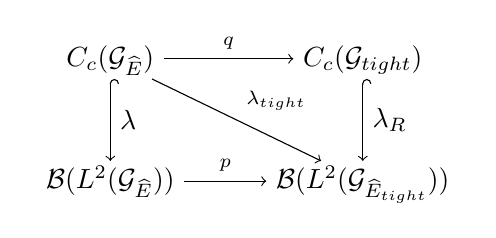
\begin{tikzpicture}
\matrix(m)[matrix of math nodes,row sep=3em, column sep=3em, text height=1.5ex, text depth = 0.25ex]
{C_{c}(\G_{\E})&C_{c}(\G_{tight})\\
\mathcal{B}(L^{2}(\G_{\E}))&\mathcal{B}(L^{2}(\G_{\E_{tight}}))\\};
\path[->,font=\scriptsize]
(m-1-1) edge node[auto] {$q$} (m-1-2)
(m-2-1) edge node[auto] {$p$} (m-2-2)
(m-1-1) edge node[auto] {$\lambda_{tight}$} (m-2-2);
\path[right hook->]
(m-1-1) edge node[auto] {$\lambda$} (m-2-1)
(m-1-2) edge node[auto] {$\lambda_{R}$} (m-2-2);

\end{tikzpicture}
\end{center}

where $\lambda_{R}$ is the left regular representation of $C_{c}(\G_{tight})$. It follows from the definition of $p$ that the bottom triangle commutes and the top triangle commutes as:
\begin{equation*}
\lambda_{x}(f) =\sum_{t \in \text{Max(S)}} f_{t}(x)\lambda_{x}(1_{tt^{*}}\delta_{t}) = \lambda_{x}(qf)
\end{equation*}
For each $x \in \E_{tight}$. Hence:
\begin{equation*}
\Vert qf \Vert_{r} = \sup_{x \in \E_{tight}} \lbrace \Vert \lambda_{x}(qf) \Vert \rbrace = \sup_{x \in \E_{tight}} \lbrace \Vert \lambda_{x}(f) \Vert \rbrace \leq \Vert \lambda(f) \Vert = \Vert f \Vert_{r}
\end{equation*}
and so $q$ is contractive (and therefore continuous).
 
Now to consider (2). It is enough to compute the result of products of elements of the form $f_{s}\delta_{s}$ for some $s \in \text{Max(S)}$. We then check the following two identities:


\begin{enumerate}[I]
\item $q(f_{s}\delta_{s} \Xst f_{t}\delta_{t}) = q(f_{s}\delta_{s})\Xst q(f_{t}\delta_{t})$
\item $(q(f_{s}\delta_{s}))^{*}=q((f_{s}\delta_{s})^{*})$
\end{enumerate}


To see (I) compute on a single element:
\begin{eqnarray*}
(f_{s}\delta_{s} \Xst f_{t}\delta_{t})([st,\phi])=f_{s}(\widehat{\rho}_{t}(\phi))f_{t}(\phi)
\end{eqnarray*}
Apply $q$:
\begin{eqnarray*}
q(f_{s}\delta_{s} \Xst f_{t}\delta_{t})([st,\phi])= (f_{s}\delta_{s} \Xst f_{t}\delta_{t})|_{\E_{tight}}([st,\phi]) =f_{s}(\widehat{\rho}_{t}(\phi))f_{t}(\phi)
\end{eqnarray*}
For all $[st,\phi] \in \G_{\E_{tight}}$. Then compute the right hand side: 
\begin{eqnarray*}
(q(f_{s}\delta_{s}) \Xst q(f_{t}\delta_{t}))([st,\phi])=f_{s}|_{\E_{tight}}(\widehat{\rho}_{t}(\phi))f_{t}|_{\E_{tight}}(\phi)
\end{eqnarray*}
Which matches for each $[st,\phi] \in \G_{\E_{tight}}$. 

To prove (II) we need to compute on a single element, where $(f_{s}\delta_{s})^{*}=\alpha_{s^{*}}(\overline{f_{s}})\delta_{s^{*}}$:

\begin{eqnarray*}
q((f_{s}\delta_{s})^{*})([s^{*},x])& = &\alpha_{s^{*}}(\overline{f_{s}})_{\E_{tight}}(x)\\
& = & \overline{f}(\widehat{\rho}_{s}(x)) \\ & = & \overline{f(\widehat{\rho}_{s}(x))} \\ & = & \overline{q(f)}(\widehat{\rho}_{s}(x)) \\ & = &  \alpha_{s^{*}}(\overline{q(f)})(x)
\end{eqnarray*}
Where the above holds for all $x \in \E_{tight}$ where the function $f_{s}$ is defined at $\widehat{\rho}_{s}(x)$ as required.

As $q$ is a continuous *-homomorphism, it extends to the completions.
\end{proof}

\subsection{Applying the machinery}\label{sect:S1-a}
We encode the norm estimations required for the proof of Theorem \ref{thm:PV1} in the following Lemma:
\begin{lemma}\label{lem:L3}
Let $S$ be F-inverse and let $K \subset \text{Max(S)}$ such that $K$ is finite and $T=\sum_{t \in K} a_{t}\lambda(1_{tt^{*}}\delta_{t})$ such that $a_{t}$ is the constant function that has value $a_{t}$ on $D_{tt^{*}}$. Then $\Vert T \Vert = \Vert qT \Vert$
\end{lemma}
\begin{proof}
It is immediate that $\Vert T \Vert \geq \Vert qT \Vert$ as $q$ is contractive. We arrive at the other inequality by applying Corollary \ref{cor:C1}.
\begin{eqnarray*}
\Vert T \Vert_{L^{2}(\mathcal{G}_{x})} = \Vert \sum_{t \in K} a_{t}\lambda_{x}(1_{tt^{*}}\delta_{t}) \Vert_{L^{2}(\mathcal{G}_{x})} = \Vert \sum_{t \in K} a_{t}Q_{x}\lambda_{\infty}(1_{tt^{*}}\delta_{t})Q_{x}^{*} \Vert_{L^{2}(\mathcal{G}_{x})} \\
= \Vert Q_{x}(\sum_{t \in K} a_{t}\lambda_{\infty}(1_{tt^{*}}\delta_{t}))Q_{x}^{*} \Vert_{L^{2}(\mathcal{G}_{x})} = \Vert Q_{x}(qT)Q_{x}^{*} \Vert_{L^{2}(\mathcal{G}_{x})} \leq \Vert qT \Vert_{L^{2}(\mathcal{G}_{\infty})}.
\end{eqnarray*}
This holds for every $x \in E$ and so by  $\Vert T \Vert = \Vert \lambda(T) \Vert = \sup \lbrace \Vert \lambda_{x}(T) \Vert : x \in E \rbrace \leq \Vert qT \Vert$. This gives the desired equality.  
\end{proof}

We remark here that if $S$ is F-inverse then minimal elements do not play a role in the ultrafilters, which was the reason for removing them when $S$ had a zero. Additionally, in this instance the groupoid $\G_{tight}$ is just the maximal group homomorphic image $G$. 

\begin{theorem}\label{thm:PV1}
Let $S$ be an F-inverse monoid, let $\G_{\E}$ be its universal groupoid, with $U \subset \E$ the compliment of $\E_{tight}$. Let $G$ be its maximal group homomorphic image. Then we have the following short exact sequence of $C^{*}$-algebras:
\begin{equation*}
0 \rightarrow C^{*}_{r}(\G_{U}) \rightarrow C^{*}_{r}(\G_{\E}) \rightarrow C^{*}_{r}(G) \rightarrow 0
\end{equation*}
\end{theorem}
\begin{proof}
Denote by $A$ the algebra $C_{c}(\G_{U})$. We know that we have a surjective *-homomorphism $q$ from $C^{*}_{r}(\G_{\E})$ to $C^{*}_{r}(G)$, we just need to see that the kernel of this map is $\overline{A}$. The set $\overline{A}$ is contained in the kernel as elements in $A$ are sums of functions with value at $1_{E}=\infty \in \widehat{E}$ of zero and projection onto this value (i.e applying q) will send the entire element to $0 \in C^{*}_{r}(G)$. So it is enough to show that $A$ is dense in the kernel.

First consider finite sums. Let $f \in C_{c}(\mathcal{G_{\E}})$. We need to show that if $qf=0$ then $ f \in A$.

$f$ has the form:
\begin{equation*}
f=\sum_{s \in S} f_{s}\delta_{s} \mbox{ where } f_{s}\in C(D_{ss^{*}})
\end{equation*}
With only finitely many non-zero terms. This can be viewed concretely on $L^{2}(\mathcal{G}_{\E})$ using
\begin{equation*}
\lambda(f)=\sum_{s \in S} f_{s}\lambda(1_{ss^{*}}\delta_{s})
\end{equation*}
As $S$ is F-inverse we can reduce this sum using the observation that for each $s \in S$ we can write the term $f_{s}\delta_{s}$ as $f_{s}\chi_{s}\delta_{t_{s}}$ where $t_{s}$ is the maximal element above $s$. So for each $t \in \text{Max(S)}$ we can define $f^{'}_{t}=\sum_{s \leq t}f(s)\chi_{s}$ and then
\begin{equation}\label{Eq1}
\lambda(f)=\sum_{t \in \text{Max(S)}} f^{'}_{t}\lambda(1_{tt^{*}}\delta_{t})
\end{equation}
(\ref{Eq1}) is in the kernel of $q$ if and only if each $f^{'}_{t}(\infty)=0$ for every $t \in \text{Max(S)}$ that is if and only if $\lambda(f) \in A$.

Now let $T$ be an element of $C^{*}_{r}(\G_{\E})$ such that $qT=0$. Then we need to show $T$ can be approximated by finite sums that lie in $A$. Let $T_{n}$ be finite sums in $C_{c}(\mathcal{G}_{\E})$ with $T_{n} \rightarrow T$. Without loss of generality, these $T_{n}$ have the following form for some finite $K_{n} \subset \text{Max(S)}$:
\begin{equation*}
T_{n}=\sum_{t \in K_{n}} f^{n}_{t}\lambda(1_{tt^{*}}\delta_{t})
\end{equation*}
then $qT_{n} = \sum_{t \in K_{n}} f^{n}_{t}(\infty)\lambda_{\infty}(1_{tt*}\delta_{t})$. Define a pullback of $qT_{n}$:
\begin{equation}
S_{n} = \sum_{t \in K_{n}} a^{n}_{t}\lambda(1_{tt*}\delta_{t}) \in C_{c}(\mathcal{G})
\end{equation}
Where $a^{n}_{t}$ is the constant function on $D_{tt^{*}}$ with value $f_{t}^{n}(\infty)$. It is clear that $qS_{n}=qT_{n}$ and using Lemma \ref{lem:L3} we have that $\Vert S_{n} \Vert = \Vert qS_{n} \Vert = \Vert qT_{n} \Vert$ so $\Vert S_{n} \Vert \rightarrow 0$\\
\\
Let $U_{n}=(T_{n}-S_{n})$. Then $U_{n} \in A$ and $U_{n}=(T_{n}-S_{n}) \rightarrow (T-0)=T$, whence $A$ is dense in $ker(q)$.
\end{proof} 

\section{A similar sequence for 0-F-inverse monoids}\label{sect:S2}
In this section we consider a generalisation of Theorem \ref{thm:PV1} to strongly 0-F-inverse monoids under some light conditions, and we proceed by considering saturated subsets of the unit space as defined in Chapter 2. Clearly, subsets that are invariant under the action of $S$ are also saturated. The following Lemma outlines the connections between saturation and Morita enveloping actions.

\begin{lemma}\label{Lem:Cut}
Let $\G$ be a \'etale locally compact Hausdorff groupoid with a (T,C,F)-cocycle $\rho$ to $\Gamma$. Then the relation $\sim$ used in constructing the Morita envelope of $\G^{(0)}$ on $\G^{(0)} \times \Gamma$ preserves saturated subsets of $\G^{(0)}$
\end{lemma}
\begin{proof}
Let $U$ be a saturated subset of $\G^{(0)}$ and let $x \in U$, $y \in U^{c}$. Assume for a contradiction that $(x,g) \sim (y,h)$ in $\G^{(0)} \times \Gamma$. Then there exists a $\gamma$ $\in \G$ such that $s(\gamma)=x$, $r(\gamma)=y$ and $\rho(\gamma)=g^{-1}h$, but as $U$ is saturated no such $\gamma$ exists. 
\end{proof}

Additionally, as we have no obvious group to consider, we introduce a universal one:

\begin{definition}
Let $S$ be an inverse semigroup. Then the \text{universal group} of $S$, denoted by $U(S)$, is the group generated by the elements of $S$ with relations $s\cdot t = st$ if $st \not = 0$.
\end{definition}

The map that sends $s \in S$ to $s \in U(S)$ is a partial homomorphism that is universal for partial homomorphism onto groups. It also induces a prehomomorphism $S \rightarrow U(S)^{0}$. An inverse monoid $S$ is strongly $0$-E-unitary if and only if this prehomomorphism is idempotent pure.

Recall that a group $G$ is said to be \textit{K-exact} if for every short exact sequence of $G$-$C^{*}$-algebras
\begin{equation*}
0 \rightarrow A \rightarrow B \rightarrow C \rightarrow 0
\end{equation*}
the corresponding sequence:
\begin{equation*}
0 \rightarrow A\rtimes_{r}G \rightarrow B\rtimes_{r}G \rightarrow C\rtimes_{r}G \rightarrow 0
\end{equation*}
is exact at the level of K-theory groups (i.e gives rise to a long exact sequence in K-theory).

\begin{theorem}\label{thm:PV2}
Let $S$ be a strongly $0$-F-inverse monoid with universal group $G:=U(S)$. If $G$ is infinite and $K$-exact then the sequence:
\begin{equation*}
0 \rightarrow C^{*}_{r}(\G_{\U}) \rightarrow C^{*}_{r}(\G_{\E}) \rightarrow C^{*}_{r}(\G_{\E_{tight}}) \rightarrow 0
\end{equation*}
is exact at the level of K-theory.  
\end{theorem}
\begin{proof}
We begin by using either Theorem \ref{Thm:IT2-a} or \ref{Thm:IT2} to construct a transformation groupoid $Y_{\E}\rtimes G$ and a Morita equivalence between $\G_{\E}$ and $Y_{\E}\rtimes G$. We can repeat this process for both $\E_{tight}$ and $U:=\E_{tight}^{c}$, and by Lemma \ref{Lem:Cut} and the fact that $\E_{tight}$ is closed in $\E$ we can conclude that we have a natural sequence of commutative $C^{*}$-algebras:
\begin{equation*}
0 \rightarrow C_{0}(Y_{U}) \rightarrow C_{0}(Y_{\E}) \rightarrow C_{0}(Y_{\E_{tight}}) \rightarrow 0
\end{equation*}
each of which is a $G$-algebra. We now act by the reduced cross product, which produces a sequence of $C^{*}$-algebras:
\begin{equation*}
0 \rightarrow C_{0}(Y_{U})\rtimes_{r}G \rightarrow C_{0}(Y_{\E})\rtimes_{r}G \rightarrow C_{0}(Y_{\E_{tight}})\rtimes_{r}G \rightarrow 0.
\end{equation*}
This may not be exact in the middle term. However by K-exactness of $G$ it is exact at the level of K-theory, so consider exact sequence:
\begin{equation*}
\xymatrix@=1em{...\ar[r] & K_{0}(C_{0}(Y_{U})\rtimes_{r} G) \ar[r]& K_{0}(C_{0}(Y_{\E})\rtimes_{r} G) \ar[r]& K_{0}(C_{0}(Y_{\E_{tight}})\rtimes_{r} G)\ar[r] & ...\\
...\ar[r] & K_{0}(C^{*}_{r}(\G_{\U})) \ar[r]\ar[u]^{\ucong}& K_{0}(C^{*}_{r}(\G_{\E})) \ar[r]\ar[u]^{\ucong}& K_{0}(C^{*}_{r}(\G_{\E_{tight}})) \ar[r]\ar[u]^{\ucong}& ...}
\end{equation*}
where the isomorphisms are induced by the Morita equivalences given by Theorems \ref{Thm:IT2-a} and \ref{Thm:IT2}. This concludes the proof.
\end{proof}

\section{Globalisation and Gromov monster groups.}\label{sect:S5}
As a final application of these results we consider Gromov monster groups and their failure to be $C^{*}$-exact. To use the techniques from the previous sections we require some more technology:

\begin{definition}
Let $X$ be a set and let $\mathcal{E}$ be a collection of subsets of $X \times X$. If $\mathcal{E}$ has the following properties:
\begin{enumerate}
\item $\mathcal{E}$ is closed under finite unions;
\item $\mathcal{E}$ is closed under taking subsets;
\item $\mathcal{E}$ is closed under the induced product and inverse that comes from the groupoid product on $X \times X$.
\item $\mathcal{E}$ contains the diagonal
\end{enumerate}
Then we say $\mathcal{E}$ is a \textit{coarse structure} on $X$ and we call the elements of $\mathcal{E}$ \textit{entourages}. If in addition $\mathcal{E}$ contains all finite subsets then we say that $\mathcal{E}$ is \textit{weakly connected}.
\end{definition}

For a given family of subsets $\mathcal{S}$ of $X \times X$ be can consider the smallest coarse structure that contains $\mathcal{S}$. This is the coarse structure generated by $\mathcal{S}$. We can use this to give some examples of coarse structures.

\begin{example}\label{ex:MCS}
Let $X$ be a metric space. Then consider the collection $\mathcal{S}$ given by the $R$-neighbourhoods of the diagonal in $X\times X$; that is, for every $R>0$ the set:
\begin{equation*}
\Delta_{R}=\lbrace (x,y) \in X \times X | d(x,y)\leq R \rbrace
\end{equation*}
Then let $\mathcal{E}$ be the coarse structure generated by $\mathcal{S}$. This is called the \textit{metric coarse structure} on $X$. It is a uniformly locally finite proper coarse structure that is weakly connected when $X$ is a uniformly discrete bounded geometry (proper) metric space.
\end{example}

\begin{definition}
Let $X$ be a coarse space with a coarse structure $\mathcal{E}$ and consider $\mathcal{S}$ a family of subsets of $\mathcal{E}$. We say that $\mathcal{E}$ is generated by $\mathcal{S}$ if every entourage $E \in \mathcal{E}$ is contained in a finite union of subsets of $\mathcal{S}$.
\end{definition}

In the situation that $X$ admits a transitive $G$-action by translations, the group action coarse structure generates the metric coarse structure. 

To build a groupoid from the metric coarse structure on $X$ we consider extensions of the pair product on $X \times X$. The most natural way to do this is by making use of the entourages arising from the metric. The approach to this problem is through the following lemma, which is Corollary 10.18 of\cite{MR2007488}:

\begin{lemma}\label{Lem:CorRoe}
Let $X$ be a uniformly discrete bounded geometry metric space and let $E$ be any entourage. Then the inclusion $E \rightarrow X \times X$ extends to an injective homeomorphism $\overline{E} \rightarrow \beta X \times \beta X$, where $\overline{E}$ denotes the closure of $E$ in $\beta(X \times X)$.
\end{lemma}
Now we can make the definition of the coarse groupoid $G(X)$:
\begin{theorem}(\cite[Theorem 10.20]{MR2007488})
Let $X$ be a coarse space with uniformly locally finite, weakly connected coarse structure $\mathcal{E}$. Define $G(X):=\cup_{E\in \mathcal{E}}\overline{E}.$ Then $G(X)$ is a locally compact, \'etale groupoid with the induced product, inverse and topology from $\beta X \times \beta X$.
\end{theorem}
As we are considering the metric coarse structure we can reduce this to considering only generators:
\begin{equation*}
G(X):=\bigcup_{R>0}\overline{\Delta_{R}}
\end{equation*}
The following is an integral part of \cite{MR1905840} and proofs of the quoted results can be found in \cite{MR2007488}.
\begin{theorem}
Let $X$ be a uniformly discrete bounded geometry metric space. Then following hold:
\begin{enumerate}
\item $G(X)$ is an \'etale locally compact Hausdorff principal topological groupoid with unit space $G(X)^{(0)}=\beta X$. \cite[Theorem 10.20]{MR2007488}\cite[Proposition 3.2]{MR1905840};
\item $C^{*}_{r}(G(X))$ is isomorphic to the uniform Roe algebra $C^{*}_{u}(X)$. \cite[Proposition 10.29]{MR2007488};
\item The coarse Baum-Connes conjecture for $X$ is equivalent to the Baum-Connes conjecture for $G(X)$ with coefficients in $\ell^{\infty}(X,\mathcal{K})$. \cite[Lemma 4.7]{MR1905840}.
\end{enumerate}
\end{theorem}

When $X$ has a countable translation structure we can say even more about the coarse groupoid.

\begin{lemma}\label{Lem:CG}
The coarse groupoid $G(X) \cong \beta X \rtimes \G(\mathcal{T}).$
\end{lemma}
\begin{proof}
We observe that the set of $[t_{g},\widehat{D}_{t_{g}^{*}t_{g}}]$ covers $G(X)$; hence the collection $\mathcal{T}$ forms an admissible psuedogroup in the terminology of \cite{MR1905840}. The groupoid it generates is $\G_{\X}$. Then the result follows from Lemma 3.3b) of \cite{MR1905840}.
\end{proof}

We make precise the definition of a Gromov monster group that we will use for the remainder of the paper.

\begin{definition}
A finitely generated discrete group $\Gamma$ is a \textit{Gromov monster group} if there exists a large girth expander with vertex degree uniformly bounded above $X$ and a coarse embedding $f: X \hookrightarrow \Gamma$. 
\end{definition}

These groups were shown to exist by Gromov \cite{MR1978492}, with a detailed proof by Arzhantseva, Delzant \cite{exrangrps}. The construction is technical and we require no details beyond those presented in the definition.

In this section we connect the globalisation of the coarse groupoid with the ideas of Higson, Willett and Yu from \cite{higsonpreprint},explg1} concerning the $C^{*}$-algebraic construction of the coefficients for which a Gromov monster group fails to have the Baum-Connes assembly map an isomorphism.

We proceed first by anaylzing the situation from \cite[Section 8]{explg1}. The primary idea is to globalise  $C^{*}X$ in $C^{*}G$. Fix a left invariant proper metric on $G$.

Let $X_{n}:=N_{n}(X)\subset G$. Then we can form the $C^{*}$-algebras $\ell^{\infty}(X_{n}) \subseteq \ell^{\infty}(G)$. Being commutative algebras in this case, we could consider the dual picture by taking spectra, getting $C_{0}(\widehat{X_{n}}) \subset C(\beta G)$. It is clear that $X_{n} \subset X_{n+1}$, so the algebras $\ell^{\infty}(X_{n}) \subset \ell^{\infty}(X_{n+1})$. The remark here is that the inclusion of $X_{n} \subset G$ is not $G$-equivariant, but the system is $G$-equivariant; the action of $G$ on $X_{n}$ on the right by translations will send points in $X_{n}$ into a most $X_{n+l(g)}$ for each $g \in G$. Hence, the limit of the $\ell^{\infty}(X_{n})$ over $n$ is a $G$-algebra, and so we can form the semidirect product algebra $(\lim_{n}\ell^{\infty}(X_{n}))\rtimes_{r} G$. Lemma 8.4 from \cite{explg1} provides us the following isomorphisms:

\begin{lemma}\label{lem:GMG}
Let $X_{n}$ as above. Then $(\lim_{n}\ell^{\infty}(X_{n}))\rtimes G \cong \lim_{n} C^{*}_{u}(X_{n})$ and $(\lim_{n}\ell^{\infty}(X_{n},\mathcal{K}))\rtimes G \cong \lim_{n} C^{*}(X_{n})$.\qed
\end{lemma}

Let the coefficients $\lim_{n}\ell^{\infty}(X_{n},\mathcal{K})$ be denoted by $A$. We appeal to the fact that each $X_{n}$ is coarsely equivalent to $X$. As these limits are functorial in coarse maps, we conclude:

\begin{proposition}
Let $G$ be a Gromov monster group and $X$ the coarsely embedded large girth expander. Then we have $A\rtimes_{r} G \cong C^{*}X$.\qed
\end{proposition}

The procedure we will follow will be a geometric analogue of this argument using translation structures and Theorem \ref{Thm:IT2} of Milan and Steinberg, which relies on the information about the coarse groupoid given above as well as the fact the the inverse semigroups associated to the coarse groupoid are strongly 0-F-inverse.

The approach is via Theorem \ref{thm:PV2}:

\begin{theorem}
Gromov monster groups are not $C^{*}$-exact.
\end{theorem}

To construct the complete sequence we use Lemma \ref{Lem:Cut} to get $Y_{1}:= (X \times G)/\sim$ and $Y_{3}:= (\partial\beta X \times G)/\sim$. We then get the short exact sequence of $G$-algebras:
\begin{equation*}
0 \rightarrow C_{0}(Y_{1}) \rightarrow C_{0}(Y_{2}) \rightarrow C_{0}(Y_{3}) \rightarrow 0.
\end{equation*}

Now we consider the crossed product algebras $C_{0}(Y_{i})\rtimes G$. Then the sequence above gives us some terms on K-theory: 
\begin{equation*}
\xymatrix@=1em{...\ar[r] & K_{0}(C_{0}(U)\rtimes G) \ar[r]& K_{0}(C_{0}(Z)\rtimes G) \ar[r]& K_{0}(C_{0}(Y)\rtimes G)\ar[r] & ...\\
...\ar[r] & K_{0}(\mathcal{K}) \ar[r]\ar[u]^{\ucong}& K_{0}(C^{*}_{r}(G(X))) \ar[r]\ar[u]^{\ucong}& K_{0}(C^{*}_{r}(G(X)|_{\partial\beta X})) \ar[r]\ar[u]^{\ucong}& ...}
\end{equation*}
And the bottom line is not exact on K-theory by either \cite{MR1911663}, \cite{explg1} or \cite{mypub1}. It follows therefore that the sequence:
\begin{equation*}
0 \rightarrow C_{0}(Y_{1})\rtimes_{r} G \rightarrow C_{0}(Y_{2})\rtimes_{r} G \rightarrow C_{0}(Y_{3})\rtimes_{r} G \rightarrow 0
\end{equation*}
is not exact in the middle term.
\end{proof}

This idea can be extended to connect this proof of failure to be exact to the geometric one that is outlined above from \cite{higsonpreprint,explg1}. 

We connect this geometric approach using groupoids to the analytic approach outlined in the previous section. 

\begin{proposition}\label{prop:GMG}
Let $X=X_{0}$ and $X_{n}$ as above. Then the globalisations of $G(X_{n})$ given by $B_{n}\rtimes G$ that come from the translation groupoid action of Lemma \ref{Lem:CG} are all Morita equivalent.
\end{proposition}
\begin{proof}
As $X_{0}$ is coarsely equivalent to $X_{n}$ for all $n$, it follows that $G(X)$ is Morita equivalent to $G(X_{n})$ for all $n$. Using Lemma \ref{Lem:CG} we can see that each of the groupoids $G(X_{n})$ is isomorphic to a transformation groupoid $\beta(X_{n}) \rtimes \G_{\X_{n})$ and therefore admits a (T,C,F)-cocycle onto the monster group $G$. Using Theorem \ref{Thm:IT2-a} (or Theorem \ref{Thm:IT2}) we can conclude that each $G(X_{n})$ is also Morita equivalent to $B_{n}\rtimes G$. Subsequently $B_{n}\rtimes G$ are Morita equivalent for each $n$, induced by the natural inclusions that extend $B_{n} \rightarrow B_{n+1}$.  
\end{proof}

Lemma \ref{lem:GMG} is naturally a corollary to Proposition \ref{prop:GMG}.

\subsection{A proof of the Baum-Connes conjecture for certain coefficients of a Gromov Monster group.}

We extend the ideas in the previous section using the results from \cite{mypub1}. The authors prove that the boundary groupoid $G(X)|_{\partial\beta X}$ of a large girth sequence with uniformly bounded vertex degree decomposes as $\partial\beta X \rtimes \G_{\widehat{X}}$, where $\G_{\widehat{X}}$ has the Haagerup property. To this end we prove:

\begin{theorem}\label{Thm:MT2}
There exists a locally compact Hausdorff space $Z$ such that the groupoid $Y_{3}\rtimes G$ is Morita equivalent to $Z \rtimes F_{k}$.
\end{theorem}

We recall the information from \cite{mypub1} that is required to prove this Theorem:

\begin{proposition}\label{Prop:Outsourced}
Let $X$ be a large girth expander with vertex degree uniformly bounded above by $2k$. Then there is bounded partial action of $F_{k}$ on $X$ that gives rise to a strongly $0$-F-inverse monoid $S_{inf}$, a locally compact, Hausdorff \etale topological groupoid $\G_{\widehat{X}}$, and a groupoid decompositon of the boundary as $G(X)|_{\partial\beta X} \cong \partial\beta X \rtimes \G_{\widehat{X}$. The groupoid $\G_{\widehat{X}}$ has the Haagerup property. \qed
\end{proposition}

\begin{lemma}\label{Lem:MEFree}
The boundary groupoid $G(X)|_{\partial\beta X}$ admits a (T,C,F)-cocycle onto $F_{k}$. 
\end{lemma}
\begin{proof}
We remark that this follows directly from the fact that the coarse boundary groupoid $G(X)|_{\partial\beta X}$ has a decompostion as $\partial\beta X \rtimes \G_{\widehat{X}}$, and that $S_{inf}$ is strongly $0$-F-inverse.
\end{proof}

\begin{proof}(Of Theorem \ref{Thm:MT2}).
Recall from the proof of Theorem \ref{Thm:MT1} that the groupoid $G(X)|_{\partial\beta X}$ is Morita equivalent to $Y_{3}\rtimes G$. Using Lemma \ref{Lem:MEFree} we know also that $Z:=(\partial\beta X \times F_{k} )/\sim$ is a locally compact Hausdorff space, arising from a (T,C,F)-cocycle onto $F_{k}$. This enables us to again appeal to either \cite[Theorem 6.14]{Milan-Steinberg} (Theorem \ref{Thm:IT2}) or \cite[Theorem 1.8]{MR1900993} (Theorem \ref{Thm:1.8}) to conclude that $G(X)|_{\partial\beta X}$ is Morita equivalent to $Z\rtimes F_{k}$. The Theorem then follows from transitivity of Morita equivalence.
\end{proof}

Theorem \ref{Thm:MT2} has an important corollary, as the Baum-Connes conjecture with coefficients is a Morita invariant:

\begin{corollary}
The Baum-Connes conjecture for $G$ with coefficients in any $(Y_{3}\rtimes G)$-$C^{*}$-algebra is an isomorphism.\qed
\end{corollary}

\bibliography{ref.bib}

\end{document}
